% !TeX spellcheck = en_US
\section{Problem 7}
Let an activation function be
\begin{equation}
S(x) = \left\{
\begin{array}{cc}
	x^k & x>L\\[1mm]
	x^k \dfrac{\left(L+x\right)^m}{\left(L+x\right)^m + \left(L-x\right)^m} & \left|x\right| \le L\\[1mm]
	0 & x < -L
\end{array}
\right.
\end{equation}
This function has some parameters $k,L,m$ called hyperparameters. Using them, this function can approximate others.
\subsection{Swish approximation}
%Swish: $k=1, \ L=2e, \ m=e$\\
In order for our activation function to approximate Swish, we have to see the latter first.
Swish's function is 
\[
S(x) = \dfrac{x}{1+e^{-x}} = x\dfrac{e^x}{1+e^x}
\]
and is plotted in figure~\ref{fig:prob7_swish}. In order to determine the parameters, we have to take a look in the plotted function. When $x>0$, Swish seems to be almost $y=x$, thus $k=1$. If we look at $x<0$, we can se that Swish curves until it settles back to 0.
That point $x_1$ where $Swish (x_1) = 0$ is parameter $L$. Trying multiple values, we opted with $2e$ as this gives the smaller error in that region.


\begin{figure}[H]
	\centering
	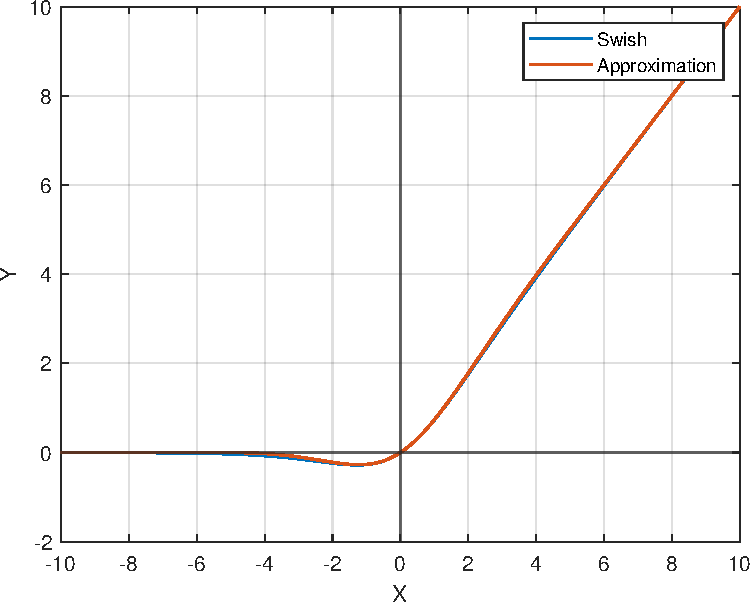
\includegraphics[width=.5\textwidth]{../Problem 7/prob7_swish.pdf}
	\caption{}
	\label{fig:prob7_swish}
\end{figure}

Sigmoid: $k=0, \ L=2e, \ m=e$.\\
ReLU: $k=1, \ L=0, \ m=0$\\
ELU: $k=, \ L=, \ m=$.